% !TeX spellcheck = it_IT
\newpage
\section{Progettazione}
Progettare una BD significa definire lo \textbf{schema globale} dei dati, i \textbf{vincoli di integrità} e le \textbf{operazioni} delle applicazioni allo scopo di prepararsi alla realizzazione. Si articola in tre fasi:
\begin{enumerate}
	\item \textbf{Analisi dei requisiti}:
	\begin{itemize}
		\item Analizza il sistema esistente e raccoglie \textbf{requisiti informali}
		\item Elimina \textbf{ambiguità}, \textbf{imprecisioni} e \textbf{disuniformità} cercando sinonimi e omonimi e unificandoli
		\item Raggruppa le frasi relative a diverse categorie di \textbf{dati}, \textbf{vincoli}, e \textbf{operazioni}
		\item Definisce un \textbf{glossario}
		\item Disegna lo \textbf{schema di settore}
		\item Specifica le \textbf{operazioni} e ne verifica la \textbf{coerenza} con i dati
	\end{itemize}
	\item \textbf{Progettazione}:
	\begin{itemize}
		\item Concettuale, logica e fisica dei dati. Identificare \textbf{classi} (e gli attributi e tipi), associazioni (e le loro proprietà), elencare le \textbf{chiavi}, individuare le \textbf{sottoclassi} e le \textbf{generalizzazioni}
		\item Delle applicazioni
	\end{itemize}
	\item \textbf{Realizzazione}
\end{enumerate}

\subsection{Documentazione}
Dato che il linguaggio naturale è pieno di \textbf{ambiguità} è fondamentale evitarle. Questo è possibile con l'aiuto delle seguenti regole per scrivere una buona \textbf{documentazione}:
\begin{itemize}
	\item Studiare e comprendere il sistema informativo e i bisogni di tutti i settori dell'organizzazione
	\item Scegliere il corretto \textbf{livello di astrazione}
	\item \textbf{Standardizzare} la struttura delle frasi
	\item \textbf{Suddividere} le frasi articolate
	\item \textbf{Separare} le frasi sui dati da quelle sulle funzioni
\end{itemize}

\begin{example}[Società di formazione]
	Si vuole realizzare una base di dati per una società che eroga corsi, di cui vogliamo rappresentare i dati dei	\textcolor{red}{partecipanti} ai corsi e dei docenti. Per gli \textcolor{red}{studenti} (circa 5000), identificati da un codice, si vuole memorizzare il codice fiscale, il cognome, l'età, il sesso, il \textcolor{darkgreen}{luogo} di nascita, il nome dei loro attuali datori di lavoro, i \textcolor{darkgreen}{posti} dove hanno lavorato in precedenza insieme al periodo, l'indirizzo e il \textcolor{lightblue}{numero di telefono}, i corsi che hanno frequentato (i corsi sono in tutto circa 200) e il giudizio finale.\\
	Rappresentiamo anche i \textcolor{brown}{seminari} che stanno attualmente frequentando e, per ogni giorno, i \textcolor{darkgreen}{luoghi} e le ore dove sono tenute le lezioni. I \textcolor{brown}{corsi} hanno un codice, un titolo e possono avere varie \textcolor{brown}{edizioni} con date di inizio e fine e numero di partecipanti. Se gli \textcolor{red}{studenti} sono liberi professionisti, vogliamo conoscere l'area di interesse e, se lo possiedono, il titolo. Per quelli che lavorano alle dipendenze di altri, vogliamo conoscere invece il loro livello e la posizione ricoperta. \\
	Per gli insegnanti (circa 300), rappresentiamo il cognome, l'età, il \textcolor{darkgreen}{posto} dove sono nati, il nome del
	corso che insegnano, quelli che hanno insegnato nel	passato e quelli che possono insegnare. Rappresentiamo anche tutti i loro \textcolor{lightblue}{recapiti telefonici}. I docenti possono essere dipendenti interni della società o collaboratori esterni.\\\\
	
	\newpage
	Per prima cosa abbiamo evidenziato dello stesso colore i \textbf{sinonimi} e le parole utilizzate in più \textbf{contesti} diversi in modo da poterli unificare e costruire il glossario.
	
	\begin{center}
		\begin{tabular}{|c|p{30mm}|c|c|}
			\hline
			\textbf{Termine} & \textbf{Descrizione} & \textbf{Sinonimi} & \textbf{Collegamenti} \\
			\hline
			Partecipante & Persona che partecipa ai corsi & Studente & Corso, società \\
			\hline
			Docente & Docente dei corsi. Può essere esterno & Insegnante & Corso \\
			\hline
			Corso & Corso organizzato dalla società. Può avere più edizioni. & Seminario & Docente \\
			\hline
			Datori & Ente presso cui i partecipanti lavorano o hanno lavorato. & Posti & Partecipante \\
			\hline			 
		\end{tabular}
	\end{center}
	Procediamo poi trovando gli \textbf{attributi}  per ogni classe.\\
	\begin{center}
		\begin{tabular}{|c|}
			\hline
			\textbf{Partecipanti} \\
			\hline
			Codice \\
			\hline
			CodiceFiscale\\
			\hline
			Cognome \\
			\hline
			Nome \\
			\hline
			Genere \\
			\hline
			CittaNascita \\
			\hline
			DataNascita \\
			\hline
		\end{tabular}
		\hspace{15pt}
		\begin{tabular}{|c|}
			\hline
			\textbf{Docenti} \\
			\hline
			CodiceFiscale\\
			\hline
			Cognome \\
			\hline
			Nome \\
			\hline
			Genere \\
			\hline
			CittaNascita \\
			\hline
			DataNascita \\
			\hline
			Recapiti \\
			\hline
		\end{tabular}
		\hspace{15pt}
		\begin{tabular}{|c|}
			\hline
			\textbf{Corsi} \\
			\hline
			Codice \\
			\hline
			Titolo\\
			\hline
		\end{tabular}
		\hspace{15pt}
		\begin{tabular}{|c|}
			\hline
			\textbf{DatoriLavoro} \\
			\hline
			CodiceFiscale\\
			\hline
			Cognome \\
			\hline
			Nome \\
			\hline
			Indirizzo \\
			\hline
			Citta \\
			\hline
			Telefono \\
			\hline
		\end{tabular}
	\end{center}
	Infine definiamo le \textbf{relazioni} tra le classi.
	\begin{center}
		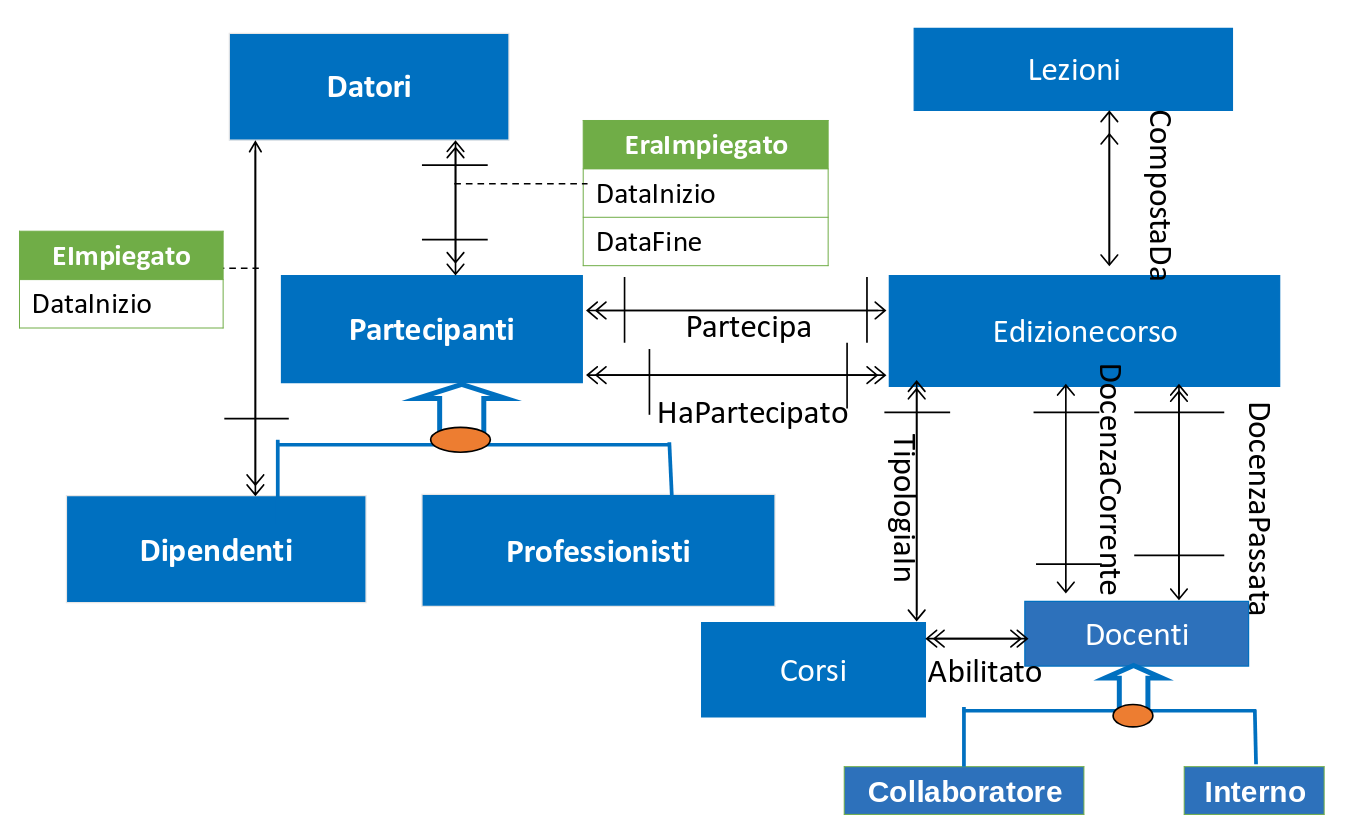
\includegraphics[scale=0.3]{esempio_prog.png}
	\end{center}
\end{example}